%%%%%%%%%%%%%%%%%%%%%%%%%%%%%%%%%%%%%%%%%%%%%%%%%%%%%%%%%%%%%%%%%%%%%%%%%%%

\documentclass{standalone}

\usepackage{amsmath}
\usepackage{mathptmx}
\usepackage{pgfplots}
\usetikzlibrary{external}
\tikzexternalize{radioactive-dice-error}
\pgfplotsset{compat=1.16}

%% IEEE uses Times Roman font, so we'll default to Times.
%% These three commands make up the entire times.sty package.
\renewcommand{\rmdefault}{ptm}
\renewcommand{\ttdefault}{pcr}
\normalfont\selectfont

\begin{document}

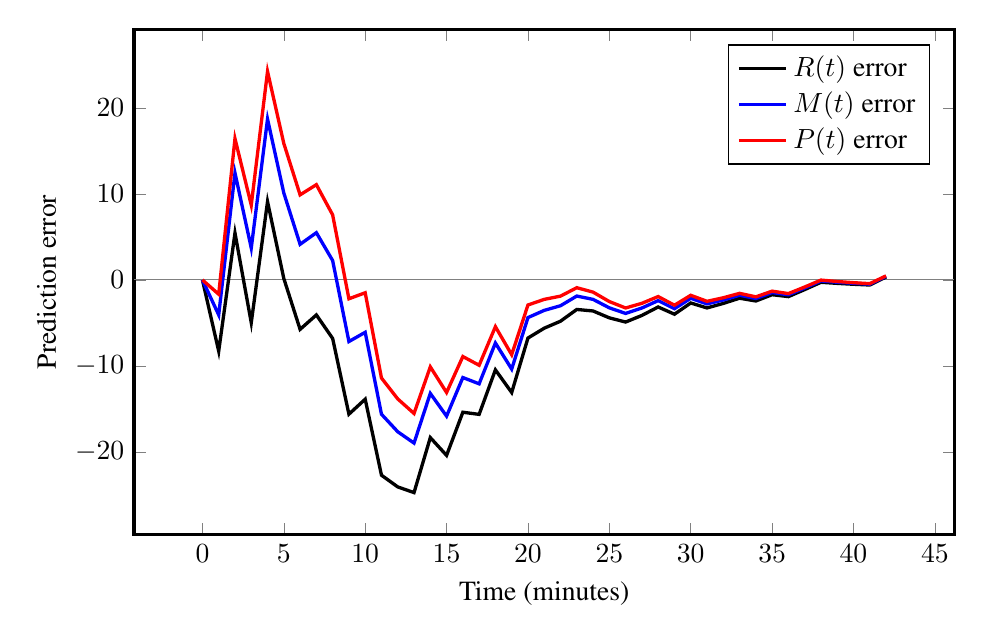
\begin{tikzpicture}
\tikzset{%%
  every mark/.append style={scale=1.0},%%
  scale=1.0%%
}
\pgfplotsset{%%
  every axis/.append style={font=\normalsize}%%
}
%%
\begin{axis}[%%
  axis line style=very thick,%%
  plotStyle/.style={very thick,mark=none},%%
  enlargelimits=true,%%
  height=8cm,%%
  legend cell align=left,%%
  legend pos=north east,%%
  width=12cm,%%
  %% x axis
  xlabel={\normalsize Time~(minutes)},%%
  %% y axis
  ylabel={\normalsize Prediction error},%%
  scaled y ticks=false,%%
  y tick label style=/pgf/number format/fixed%%
]
%%
%%
%% Horizontal line through origin.
\draw[gray,thin] ({rel axis cs:0,0}|-{axis cs:0,0}) -- ({rel axis cs:1,0}|-{axis cs:1,0});
%%
%%
%% Error for the function R(t).
\addplot[plotStyle,black] coordinates {
  (0, 0)
  (1, -8.28700000000003)
  (2, 5.45438436899985)
  (3, -4.97937553515112)
  (4, 9.10989551320859)
  (5, 0.165823049411244)
  (6, -5.75169392935214)
  (7, -4.07327514341654)
  (8, -6.80834551363935)
  (9, -15.6181227446174)
  (10, -13.8759571085708)
  (11, -22.7172151290979)
  (12, -24.080519071022)
  (13, -24.7418401627618)
  (14, -18.3426839064773)
  (15, -20.4133912403756)
  (16, -15.3924019125046)
  (17, -15.6421797622924)
  (18, -10.4623783578241)
  (19, -13.1007251993318)
  (20, -6.7620198317152)
  (21, -5.61557270113677)
  (22, -4.80135495447488)
  (23, -3.4350825584788)
  (24, -3.61241940716768)
  (25, -4.41245208535782)
  (26, -4.90056250084242)
  (27, -4.13080272675894)
  (28, -3.14785831464706)
  (29, -3.98867139087682)
  (30, -2.68378249156595)
  (31, -3.25843987494996)
  (32, -2.7335166043395)
  (33, -2.12626871252333)
  (34, -2.4509619861363)
  (35, -1.7193901364447)
  (36, -1.9413031778706)
  (37, -1.12476157408694)
  (38, -0.276429015198137)
  (39, -0.401814460441497)
  (40, -0.505472238034972)
  (41, -0.591167470322606)
  (42, 0.337987167107188)
};
\addlegendentry{$R(t)$ error}
%%
%%
%% Error for the function M(t).
\addplot[plotStyle,blue] coordinates {
  (0, 0)
  (1, -4.07100000000003)
  (2, 12.4430030409998)
  (3, 3.70911407385495)
  (4, 18.7115404482741)
  (5, 10.1134435931439)
  (6, 4.14214757140746)
  (7, 5.49375553936198)
  (8, 2.25389279656653)
  (9, -7.16815011244182)
  (10, -6.09413980478118)
  (11, -15.622370493847)
  (12, -17.6654466920818)
  (13, -18.9816779544049)
  (14, -13.2011656809757)
  (15, -15.8474793981275)
  (16, -11.3556682088066)
  (17, -12.0872270290755)
  (18, -7.34253246804268)
  (19, -10.3711761611382)
  (20, -4.38055103639844)
  (21, -3.54298589212352)
  (22, -3.00167372435631)
  (23, -1.87559774610567)
  (24, -2.26362455957384)
  (25, -3.24790529166213)
  (26, -3.89670169609552)
  (27, -3.26673444363496)
  (28, -2.40513438451515)
  (29, -3.35106390899079)
  (30, -2.13706418283381)
  (31, -2.79017460437791)
  (32, -2.33286299384114)
  (33, -1.78379851460942)
  (34, -2.15849391594589)
  (35, -1.469839191083)
  (36, -1.72854500920741)
  (37, -0.943511175955704)
  (38, -0.122132797925697)
  (39, -0.270554683647602)
  (40, -0.393882732728618)
  (41, -0.496359585223458)
  (42, 0.418489426209857)
};
\addlegendentry{$M(t)$ error}
%%
%%
%% Error for the function P(t).
\addplot[plotStyle,red] coordinates {
  (0, 0)
  (1, -1.66666666666663)
  (2, 16.4444444444446)
  (3, 8.70370370370381)
  (4, 24.2530864197532)
  (5, 15.877572016461)
  (6, 9.8979766803842)
  (7, 11.0816472336535)
  (8, 7.56803936137794)
  (9, -2.19330053218505)
  (10, -1.49441711015422)
  (11, -11.4120142584619)
  (12, -13.8433452153849)
  (13, -15.5361210128207)
  (14, -10.1134341773506)
  (15, -13.0945284811255)
  (16, -8.91210706760457)
  (17, -9.92675588967047)
  (18, -5.43896324139206)
  (19, -8.69913603449338)
  (20, -2.91594669541115)
  (21, -2.26328891284262)
  (22, -1.88607409403552)
  (23, -0.905061745029599)
  (24, -1.42088478752467)
  (25, -2.51740398960389)
  (26, -3.2645033246699)
  (27, -2.72041943722492)
  (28, -1.9336828643541)
  (29, -2.94473572029508)
  (30, -1.78727976691257)
  (31, -2.48939980576047)
  (32, -2.07449983813373)
  (33, -1.56208319844477)
  (34, -1.96840266537064)
  (35, -1.3070022211422)
  (36, -1.5891685176185)
  (37, -0.824307098015419)
  (38, -0.020255915012849)
  (39, -0.183546595844041)
  (40, -0.319622163203367)
  (41, -0.43301846933614)
  (42, 0.47248460888655)
};
\addlegendentry{$P(t)$ error}
\end{axis}
\end{tikzpicture}

\end{document}
